% !TEX program = xelatex
% Gerado por artigo/gerar_tex.py a partir de artigo/rascunho-artigo.md. Não edite à mão:
% altere o .md e rode `python artigo/gerar_tex.py --pdf`. Compila com XeLaTeX (recomendado),
% LuaLaTeX ou pdfLaTeX; no Overleaf, o arquivo latexmkrc desta pasta já seleciona o XeLaTeX.
\documentclass[12pt,a4paper]{article}
\usepackage[top=3cm,bottom=2cm,left=3cm,right=2cm,headsep=0.8cm]{geometry}
\usepackage{iftex}
\usepackage{amsmath}
\usepackage[brazilian]{babel}
\ifPDFTeX
  % pdfLaTeX: Times pelo newtx (ou pelo mathptmx, se o newtx não estiver instalado)
  \usepackage[T1]{fontenc}
  \usepackage[utf8]{inputenc}
  \IfFileExists{newtxtext.sty}{\usepackage{newtxtext,newtxmath}}{\usepackage{mathptmx}}
\else
  % XeLaTeX/LuaLaTeX: Times New Roman 12, como pedem as instruções da disciplina. Onde ela não
  % estiver instalada (Overleaf, Linux), usa a TeX Gyre Termes, clone métrico da Times do TeX Live.
  \usepackage{unicode-math}
  \IfFontExistsTF{Times New Roman}
    {\setmainfont{Times New Roman}}
    {\setmainfont{texgyretermes}[Extension=.otf, UprightFont=*-regular, BoldFont=*-bold,
       ItalicFont=*-italic, BoldItalicFont=*-bolditalic]}
  \setmathfont{texgyretermes-math.otf}
\fi
\usepackage{microtype}
\usepackage{indentfirst}  % recua também o primeiro parágrafo de cada seção (uso brasileiro)
\usepackage{graphicx}
\usepackage{calc}
\usepackage{array}
\usepackage{longtable}
\usepackage{booktabs}
\usepackage{enumitem}
\usepackage{titlesec}
\usepackage{fancyhdr}
\usepackage{xurl}
\usepackage{xcolor}
\definecolor{azul}{RGB}{25,70,140}
\usepackage[colorlinks=true, linkcolor=azul, urlcolor=azul, citecolor=azul]{hyperref}
\urlstyle{same}

% Espaçamento simples; recuo de 1,25 cm na primeira linha (ABNT), sem espaço extra entre parágrafos
\setlength{\parindent}{1.25cm}
\setlength{\parskip}{0pt plus 1pt}
\setlength{\emergencystretch}{1.5em}
\frenchspacing  % espaço simples depois do ponto, como no português
\setcounter{secnumdepth}{2}
\titleformat{\section}{\normalfont\normalsize\bfseries}{\thesection}{0.5em}{}
\titleformat{\subsection}{\normalfont\normalsize\bfseries}{\thesubsection}{0.5em}{}
\titlespacing*{\section}{0pt}{12pt}{0pt}
\titlespacing*{\subsection}{0pt}{12pt}{0pt}
\setlist[itemize]{leftmargin=1.2em, topsep=0pt, itemsep=1.5pt, parsep=0pt}
\providecommand{\tightlist}{\setlength{\itemsep}{1.5pt}\setlength{\parskip}{0pt}}

% Número da página no canto superior direito (ABNT)
\pagestyle{fancy}
\fancyhf{}
\fancyhead[R]{\footnotesize\thepage}
\renewcommand{\headrulewidth}{0pt}
\setlength{\headheight}{14.5pt}
\fancypagestyle{plain}{\fancyhf{}\fancyhead[R]{\footnotesize\thepage}}

% A Figura 1 ocupa uma página; floats grandes vão para a página seguinte à menção
\renewcommand{\floatpagefraction}{0.8}
\setlength{\LTpre}{6pt}
\setlength{\LTpost}{0pt}

% Referências: alinhadas à esquerda, espaço simples, separadas por 3 pt
\newenvironment{referencias}{\raggedright\setlength{\parindent}{0pt}\setlength{\parskip}{3pt}}{\par}
\hypersetup{pdftitle={Avaliação do desenho da Lei de Incentivo à Cultura Capixaba e proposta de avaliação de impacto}, pdflang={pt-BR}}

\begin{document}

\begin{center}
{\large\bfseries Avaliação do desenho da Lei de Incentivo à Cultura Capixaba e proposta de avaliação de impacto\par}
\vspace{6pt}
Felipe Carvalho Souza Santos\par
\vspace{3pt}
Vitória, setembro de 2026\par
\end{center}

\noindent\textbf{Resumo.} A Lei de Incentivo à Cultura Capixaba (LICC) permite que empresas contribuintes do
ICMS destinem a projetos culturais habilitados pela Secretaria da Cultura (SECULT) valores que
recuperam integralmente como crédito presumido do imposto: o Estado paga, a empresa escolhe, e o
público a quem o bem cultural se destina não entra na escolha. Neste artigo, avalia-se o desenho da
LICC: da teoria da mudança derivam-se cinco premissas, confrontadas com normas, anexos oficiais e
atas da comissão de 2022 a 2026, que orientam uma proposta de avaliação de impacto. A decisão de
financiamento não mostra orientação evidente pelo valor público: duas empresas respondem por metade
da renúncia de 2025, e o bem cultural oferecido à população confunde-se com o marketing das
empresas. A decisão se concentra em poucos atores: a habilitação qualifica sem priorizar, e o que
excede o teto é racionado pela ordem de recebimento e validação dos termos de patrocínio. Até 13\%
do valor captado em 2025 poderia remunerar captação e elaboração, projetos pequenos captam cada vez
menos, e só pessoas jurídicas contribuintes patrocinam. Propõem-se quatro perguntas de avaliação,
com estratégias, dados e poder estatístico, entre elas um experimento conjunto com decisores de
empresas.

\noindent\textbf{Palavras-chave:} incentivo fiscal à cultura; gasto tributário; patrocínio; bens públicos;
teoria da mudança; avaliação de impacto.

\section{Introdução}\label{secao-1}

A Lei estadual nº 11.246/2021 incluiu na lei do ICMS um crédito presumido correspondente ao valor
que o contribuinte destina a projetos culturais credenciados pela Secretaria da Cultura (SECULT),
com efeitos a partir de 2022 (ESPÍRITO SANTO, 2021a). A Lei de Incentivo à Cultura Capixaba (LICC)
cresceu: o teto anual de captação, o montante fixado pela SEFAZ, passou de R\$ 15 milhões em 2023
para R\$ 31 milhões em 2026.\footnote{Para 2022, a Portaria SEFAZ nº 09-R fixou R\$ 10 milhões, e a
  Portaria SEFAZ nº 83-R, de 26 de setembro, ampliou o montante em R\$ 5 milhões (DIO-ES, 2026): o
  teto de 2022 foi de R\$ 15 milhões, valor que o anexo de captação da SECULT e a lista do Portal da
  Transparência informam (ESPÍRITO SANTO, 2026), dos quais R\$ 11,5 milhões foram validados.} De
2023 a 2025, a captação esgotou o teto: os termos de patrocínio listados pela SECULT somam
exatamente o montante de cada ano (em 2025, 62 projetos validados somam R\$ 24,64 milhões, e um
ainda ``em análise na SEFAZ'' completa os R\$ 25 milhões; os números de 2025 contam os 63). A
demanda supera o teto: nos cinco ciclos de habilitação (2022-2026), 463 projetos foram autorizados a
captar, somados, R\$ 184 milhões (459 com valor válido), acima da soma dos tetos do período, de R\$
111 milhões.\footnote{Todos os números deste artigo vêm dos anexos oficiais da SECULT (``Lista de
  projetos habilitados'' e ``Recurso financeiro captado'', de 2022 a 2026), de bases públicas do
  IBGE, do Tesouro Nacional (SICONFI) e do Portal da Transparência do ES. A lista de habilitados foi
  transcrita na versão disponível em 3 set. 2026 (repositório licc.gov); a SECULT atualizou o
  arquivo em 10 set. 2026, e os status publicados podem ter mudado desde então. Dados, scripts e
  tabelas: \url{https://github.com/fcarva/aval-pol}.}

O setor cultural capixaba é pequeno para o tamanho da economia do estado: em 2024, ocupava 4,2\% dos
trabalhadores do ES, contra 5,8\% no país, a 18ª participação entre as 27 unidades da federação
(IBGE, 2025). Na economia criativa, que soma às artes atividades de mercado como design e
publicidade, o estado ficava perto da média: 8,2\% dos ocupados no 2º trimestre de 2020, contra
8,5\% no país, a 8ª posição (SECULT, 2020). O contraste sugere que o atraso está no núcleo cultural,
que a LICC financia, e não na atividade criativa como um todo. A desigualdade relevante, porém, é
interna: em 2021, 95\% da população da Região Metropolitana da Grande Vitória (RMGV) vivia em
município com cinema, contra 34\% da do interior, e metade dos municípios do interior não tinha
fundo municipal de cultura (IBGE, 2022). O problema é, assim, a baixa e desigual capacidade de
financiar a produção e a oferta cultural fora do circuito já consolidado, com causas na restrição de
financiamento de pequenos produtores, na concentração de equipamentos e na dependência de poucos
financiadores.

A avaliação da LICC se justifica por duas razões. Primeiro, trata-se de gasto público que não passa
pelo lado da despesa do orçamento: a renúncia efetiva equivale a 14\% a 21\% do gasto estadual
direto na função cultura em 2022-2025 (SECULT, 2026c; BRASIL, 2026). Segundo, quem decide o destino
do recurso é a empresa patrocinadora, e não o Estado, o que expõe a política às críticas de
concentração e de lógica de marketing feitas à Lei Rouanet (SILVA, 2017; DEKKER; RODRIGUES, 2019).

O artigo tem dois objetivos: avaliar o desenho da LICC, sem propor redesenho do mecanismo, e
estruturar uma avaliação de impacto, com desenho amostral, fontes de dados e cálculo de poder. A
\hyperref[secao-2]{seção~2} caracteriza a política, a 3 revisa a literatura, a 4 reconstrói e audita a teoria da
mudança, a 5 propõe a avaliação de impacto e a 6 conclui.

\section{Caracterização da política}\label{secao-2}

A LICC é um \textbf{gasto tributário alocado por empresas}. O proponente inscreve o projeto na
SECULT. Se o projeto for habilitado, o proponente procura uma empresa contribuinte do ICMS que
aceite patrocinar. A empresa deposita o valor numa conta do projeto e compensa até 100\% dele com o
ICMS devido, sem contrapartida financeira (ESPÍRITO SANTO, 2021b, art. 10). O \hyperref[quadro-1]{Quadro~1} resume as
regras.

\begingroup\footnotesize\renewcommand{\arraystretch}{1.15}
\phantomsection\label{quadro-1}
\begin{longtable}{@{}>{\raggedright\arraybackslash}p{(\linewidth - 4\tabcolsep) * \real{0.2121}}>{\raggedright\arraybackslash}p{(\linewidth - 4\tabcolsep) * \real{0.5152}}>{\raggedright\arraybackslash}p{(\linewidth - 4\tabcolsep) * \real{0.2727}}@{}}
\multicolumn{3}{@{}p{\linewidth}@{}}{\normalsize\raggedright \textbf{Quadro 1} -- Elementos do desenho da LICC} \\[4pt]
\toprule
Elemento & Regra vigente & Norma \\
\midrule
\endfirsthead
\multicolumn{3}{@{}l}{\normalsize\textit{Quadro 1 -- Elementos do desenho da LICC (continuação)}} \\[4pt]
\toprule
Elemento & Regra vigente & Norma \\
\midrule
\endhead
\bottomrule
\endfoot
\bottomrule
\addlinespace[2pt]
\multicolumn{3}{@{}p{\linewidth}@{}}{\raggedright \textit{Fonte}: elaboração própria a partir das normas citadas (ESPÍRITO SANTO, 2021a; 2021b; SECULT, 2022; 2023a; 2025a; 2026a).} \\
\endlastfoot
Benefício ao patrocinador & Crédito presumido de até 100\% do patrocínio, compensado com o ICMS a recolher & Lei 7.000/2001, art. 5º-B, IX; Dec.~5.035-R/2021, art. 10 \\ \addlinespace[3pt]
Teto anual & Fixado pela SEFAZ até 31/01, ampliável no exercício, limitado a 2\% do ICMS estadual do ano anterior: R\$ 15 mi em 2022 (10 mi ampliados em setembro) e 2023, 25 mi em 2024 e 2025, 31 mi em 2026 & Dec.~5.035-R/2021, art. 4º; Dec.~5.210-R/2022; portarias SEFAZ \\ \addlinespace[3pt]
Patrocinador & Pessoa jurídica contribuinte do ICMS fora do Simples Nacional, até 20\%, 15\%, 10\% ou 5\% do ICMS recolhido no ano anterior, conforme a faixa de imposto & Dec.~5.035-R/2021, arts. 2º e 10, § 1º; LC 123/2006, art. 24; IN 001/2026, art. 40 \\ \addlinespace[3pt]
Proponentes & Pessoa jurídica com finalidade cultural e sede no ES há 2 anos; até 3 inscrições por ano & Dec.~5.035-R/2021, art. 5º; IN 001/2025, art. 13 \\ \addlinespace[3pt]
Linhas e limite por projeto & Seis linhas, das linguagens artísticas ao audiovisual, sem reserva do teto por linha; até 2023, 5\% do montante anual; desde 2024, R\$ 500 mil (R\$ 1 milhão para obra em patrimônio e longa-metragem; R\$ 300 mil em primeira edição, desde 2025) & IN 002/2022 e 001/2023, art. 8º; IN 001/2025, arts. 9º e 14-16 \\ \addlinespace[3pt]
Seleção & Parecer técnico sobre nove critérios qualitativos (``atende ou não''), sem nota; o parecer favorável emite o certificado, e a comissão paritária (CAP) habilita ou não, podendo exigir ajustes & Dec.~5.035-R/2021, art. 14; IN 001/2025, arts. 37-45 \\ \addlinespace[3pt]
Alocação entre habilitados & Pela empresa patrocinadora; reservas do teto: 30\% para eventos com mais de 10 anos, 10\% para planos plurianuais, 10\% para projetos fora da RMGV, 50\% para os demais & IN 001/2025, art. 18 \\ \addlinespace[3pt]
Custos com o recurso incentivado & Captação até 10\% (R\$ 50 mil) e elaboração até 5\% (R\$ 15 mil); em 2026, despesa única de até 10\%, paga até ao proponente; divulgação até 25\%; marca do patrocinador em proporção com a do Governo & IN 001/2025, arts. 23, 27-28, 55 e 64; IN 001/2026, art. 28 \\ \addlinespace[3pt]
Contrapartidas & Ao menos cinco, de um cardápio de acesso, gratuidade, descentralização, ações afirmativas e acessibilidade & IN 001/2025, arts. 35-36 \\ \addlinespace[3pt]
Controle & Extrato no Diário Oficial a cada repasse; prestação de contas do objeto; fiscalização por amostragem & Dec.~5.035-R/2021, arts. 17-19 \\
\end{longtable}
\endgroup

Três características do arranjo pesam na avaliação. A primeira é a delegação da escolha: o Estado
define quem pode receber; a empresa define quem recebe. A segunda é a instabilidade: a SECULT edita
uma instrução normativa por ano, fechou as inscrições em meados de 2024 e alterou o fluxo em meados
de 2025 (SECULT, 2024b; 2025b); até 2024 a comissão habilitava antes da captação, e desde 2025 o
projeto só vai à comissão com patrocinador (SECULT, 2025a, arts. 41-45). A terceira é a pouca
informação publicada: os anexos não trazem dados cadastrais do proponente, o local de atuação nem
indicadores de resultado, e os inabilitados só aparecem nos extratos das atas da comissão (SECULT,
2026f).

\section{Breve revisão da literatura}\label{secao-3}

\textbf{Despesa tributária com decisão privada.} A literatura de economia da cultura trata o
incentivo fiscal como um subsídio em que o doador decide a alocação e o Tesouro paga a conta: para
Feld, O'Hare e Schuster (1983), os contribuintes americanos se tornaram ``mecenas apesar de si
mesmos'', porque financiam pela renúncia escolhas que não fazem. A justificativa econômica é o
caráter de bem público da cultura: bens públicos são consumidos em grupo, e não por indivíduos, e
por isso são ``o tecido que conecta as pessoas'' (HITZIG, 2021, tradução nossa); Buterin, Hitzig e
Weyl (2019) tratam seu financiamento como formação de comunidades e mostram que, se o valor recebido
cresce com o número de contribuintes, e não só com o total aportado, a provisão é ótima no modelo
dos autores.

\textbf{A experiência brasileira com a Lei Rouanet.} A LICC reproduz o núcleo do mecenato federal,
que acumula três décadas de debate: concentração regional no Sudeste (SILVA, 2017), concentração
persistente de patrocinadores e proponentes (COSTA; MEDEIROS; BUCCO, 2017) e um ``mercado de
patrocínios'' com intermediários e departamentos de marketing (BELEM; DONADONE, 2013). Dekker e
Rodrigues (2019) concluem que a lei beneficiou sobretudo projetos já bem-sucedidos e que não está
claro qual falha de mercado ela corrige, dúvida que vale para a LICC (\hyperref[secao-4.2]{seção~4.2}). Em 2010-2019, o
maior doador destinou 853 vezes o valor do doador médio, e o número de doadores de um projeto não se
relaciona com a parcela do aprovado que ele capta (OGAVA; GALVÃO; ADAMCZYK, 2022).

\textbf{Evidência causal.} Existem poucos trabalhos de avaliação do incentivo cultural no Brasil; as
avaliações encontradas de leis estaduais via ICMS são descritivas: em Minas Gerais, a captação pela
lei estadual concentrou-se na região metropolitana de Belo Horizonte, e municípios com museu, teatro
ou cinema tinham mais chance de captar (TEIXEIRA \emph{et al.}, 2021).

\section{Desenho da política e sua avaliação}\label{secao-4}

\subsection{Teoria da mudança}\label{secao-4.1}

A teoria da mudança da LICC (\hyperref[figura-1]{Figura~1}) segue cinco passos: propósito, cadeia causal, premissas e
riscos, hipótese causal e indicadores. Na cadeia de resultados de Gertler \emph{et al.} (2018), os
produtos estão sob controle do órgão executor; na LICC, o produto ``projeto patrocinado'' depende de
um terceiro, a empresa. Por isso a \hyperref[figura-1]{Figura~1} separa três cadeias: a entrada, o financiamento e a
entrega, e indica quem decide em cada elo.

A hipótese causal é: \emph{se} a SECULT abre a inscrição e habilita projetos culturais, e empresas
contribuintes patrocinam parte deles com o ICMS que pagariam, \emph{então} se forma um cardápio de
projetos habilitados e um conjunto de projetos patrocinados e executados, \emph{o que deveria levar}
a mais bens culturais de acesso público, executados por proponentes mais diversos e mais capazes,
\emph{que ao final melhorarão} o acesso da população à cultura e reduzirão sua desigualdade
territorial, \emph{contribuindo para} ampliar e desconcentrar a capacidade de financiar a cultura no
estado.

Cada seta da cadeia carrega uma premissa, uma condição que precisa valer para que um passo leve ao
seguinte (MAYNE, 2015). Cinco delas são tratadas como hipóteses a testar, marcadas nos elos da
\hyperref[figura-1]{Figura~1} e auditadas no \hyperref[quadro-2]{Quadro~2}. H1 (marketing): a empresa escolhe pela marca, único retorno
privado do crédito integral, sem deixar de fora bem público que a população valorizaria. H2 (decisão
concentrada): a decisão sobre recurso público segue critério público e não fica com poucos
decisores. H3 (taxa de serviço): o recurso chega ao bem cultural, e não à intermediação. H4
(exclusão): quem não tem acesso a grandes contribuintes consegue entrar. H5 (entrega): o bem
financiado não existiria sem a LICC. H1 a H4 perguntam quem decide e a que custo; H5, se o que se
financia é adicional. Há dois riscos (efeitos não esperados): o teto fixo desloca outros projetos, e
o crédito integral pode substituir o patrocínio próprio da empresa.

\begin{figure}[p]
\phantomsection\label{figura-1}
{\raggedright \textbf{Figura 1} -- Teoria da mudança da LICC\par}
\vspace{6pt}
\centering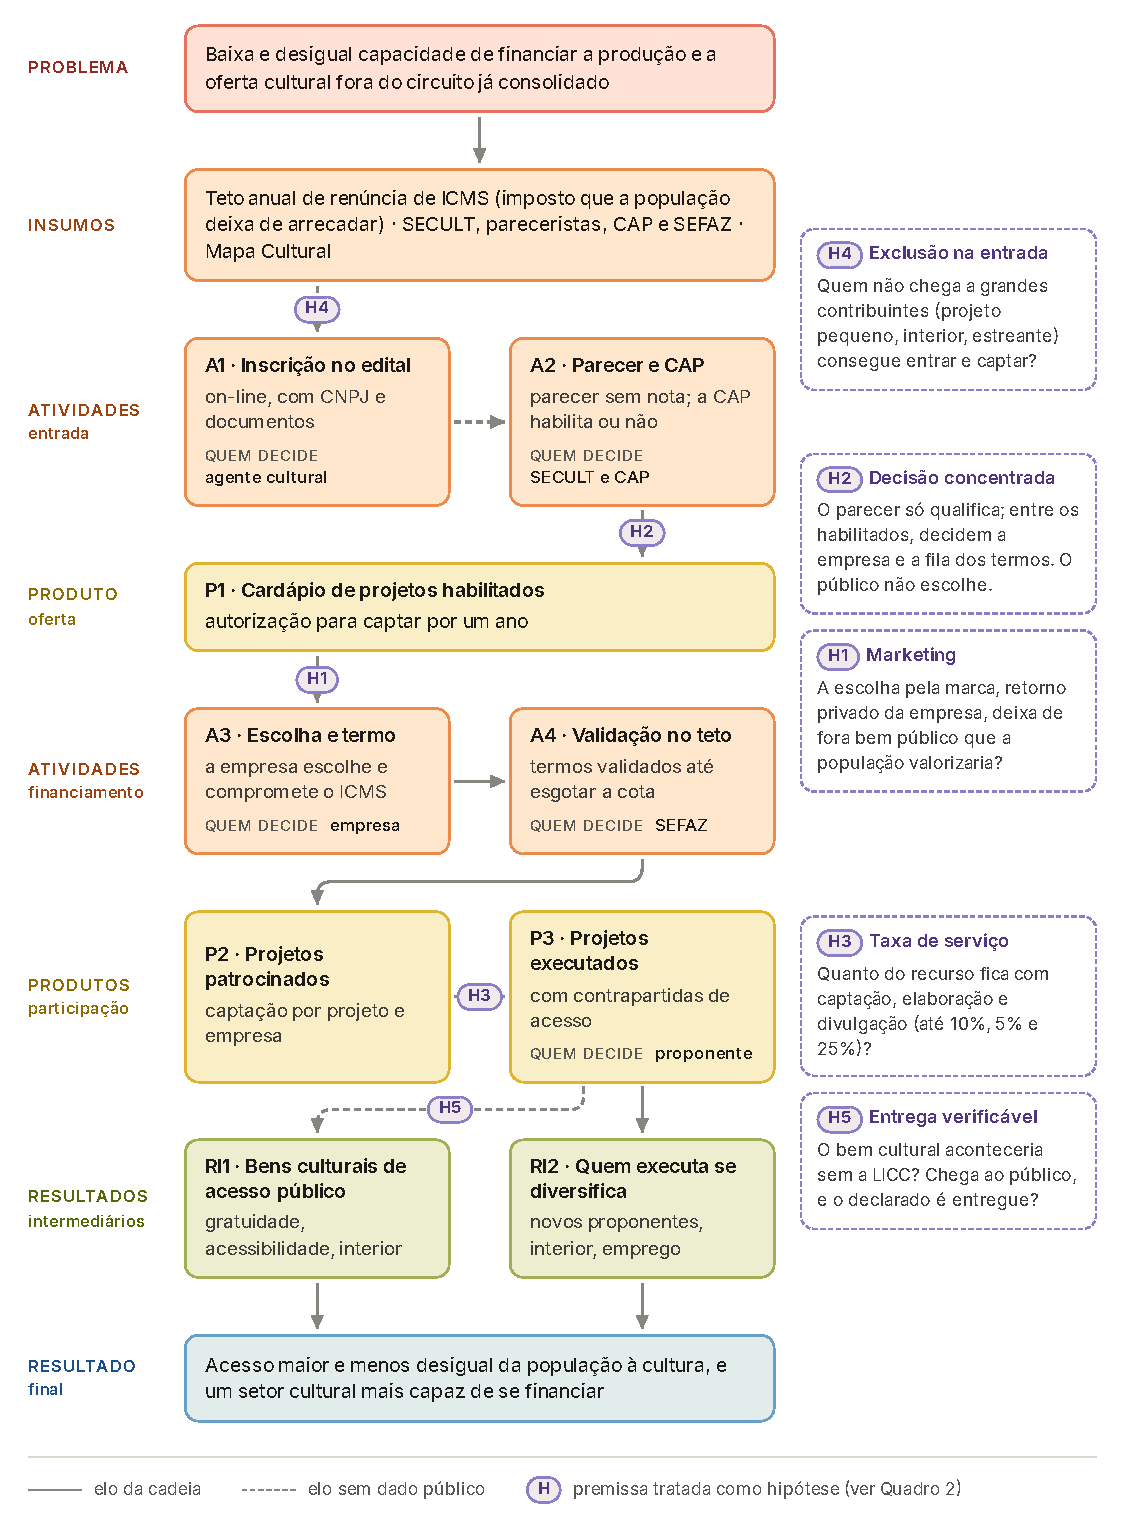
\includegraphics[width=\linewidth]{figuras/08_teoria_da_mudanca.pdf}\par
\vspace{4pt}
{\raggedright\footnotesize \textit{Fonte}: elaboração própria, no formato do J-PAL (GERTLER \emph{et al.}, 2018), com base nas normas do Quadro 1. Setas tracejadas: elos sem dado público.\par}
\end{figure}

\subsection{Avaliação do desenho}\label{secao-4.2}

Aplicam-se as perguntas usuais de avaliação de desenho: o problema está formulado? Os objetivos são
mensuráveis? Cada elo tem premissa crível e indicador? Quanto se perde ao longo da cadeia? Pelo
mecanismo de mapeamento de Williams (2020), a premissa de cada elo é confrontada com o contexto real
e classificada como sustentada, não assegurada pelo desenho, não sustentada (evidência mista) ou
indeterminada (\hyperref[quadro-2]{Quadro~2}).

\textbf{Problema e objetivos.} A lei não tem artigo de objetivos, e o decreto declara na ementa um
objetivo de produto, ``estimular a realização de projetos culturais''; suas onze finalidades de
``interesse público'', das quais o projeto atende \textbf{uma ou mais}, definem quem é elegível, não
o que a política pretende alcançar (ESPÍRITO SANTO, 2021b, art. 3º). Não há meta, magnitude esperada
nem indicador. A LICC não atende ao critério de que um programa declare resultados e magnitude
esperados (BARROS; LIMA, 2017).

\textbf{Funil de atrito e indicadores.} O funil mede, elo a elo, quantos beneficiários potenciais
chegam ao fim da cadeia (WHITE; RAITZER, 2017); suas etapas são os indicadores da cadeia, e os de
resultado são os \emph{Y} do \hyperref[quadro-3]{Quadro~3}. A \hyperref[tabela-1]{Tabela~1} mostra que ele se estreita onde não há dado: entre
os 25.441 agentes cadastrados no Mapa Cultural e os 53 a 95 proponentes habilitados por ciclo, não
se sabe quantos se inscreveram. Nas etapas observadas, a maioria passa: 68\% dos habilitados de
2022-2024 com situação resolvida captaram.

\begingroup\footnotesize\renewcommand{\arraystretch}{1.15}
\phantomsection\label{quadro-2}
\begin{longtable}{@{}>{\raggedright\arraybackslash}p{(\linewidth - 6\tabcolsep) * \real{0.1176}}>{\raggedright\arraybackslash}p{(\linewidth - 6\tabcolsep) * \real{0.2941}}>{\raggedright\arraybackslash}p{(\linewidth - 6\tabcolsep) * \real{0.4235}}>{\raggedright\arraybackslash}p{(\linewidth - 6\tabcolsep) * \real{0.1647}}@{}}
\multicolumn{4}{@{}p{\linewidth}@{}}{\normalsize\raggedright \textbf{Quadro 2} -- Premissas da teoria da mudança} \\[4pt]
\toprule
Elo & Premissa & Contexto real & Situação \\
\midrule
\endfirsthead
\multicolumn{4}{@{}l}{\normalsize\textit{Quadro 2 -- Premissas da teoria da mudança (continuação)}} \\[4pt]
\toprule
Elo & Premissa & Contexto real & Situação \\
\midrule
\endhead
\bottomrule
\endfoot
\bottomrule
\addlinespace[2pt]
\multicolumn{4}{@{}p{\linewidth}@{}}{\raggedright \textit{Fonte}: elaboração própria, no formato do mecanismo de mapeamento de Williams (2020), com base nas normas do Quadro 1, em SECULT (2026b; 2026c; 2026d), no Portal da Transparência (ESPÍRITO SANTO, 2026) e nas tabelas \href{https://github.com/fcarva/aval-pol/tree/main/analise/tabelas}{\nolinkurl{03_*.csv}}, \href{https://github.com/fcarva/aval-pol/tree/main/analise/tabelas}{\nolinkurl{07_*.csv}}, \href{https://github.com/fcarva/aval-pol/tree/main/analise/tabelas}{\nolinkurl{09_*.csv}}, \href{https://github.com/fcarva/aval-pol/tree/main/analise/tabelas}{\nolinkurl{10_*.csv}}, \href{https://github.com/fcarva/aval-pol/tree/main/analise/tabelas}{\nolinkurl{14_*.csv}} e \href{https://github.com/fcarva/aval-pol/tree/main/analise/tabelas}{\nolinkurl{16_*.csv}} de \href{https://github.com/fcarva/aval-pol/tree/main/analise/tabelas}{\nolinkurl{analise/tabelas/}}.} \\
\endlastfoot
Escolha (H1) & A escolha pela marca, único retorno privado da empresa, não deixa de fora bem público que a população valorizaria & Duas empresas somam metade da renúncia de 2025; energia e gás, 52\%. As peças de divulgação (até 25\%) trazem a marca. Recorrentes captam mais (71\% contra 57\%); 48 pares patrocinador--proponente se repetem (44\% do valor) & Não sustentada: evidência mista \\ \addlinespace[3pt]
Habilitação e validação (H2) & A decisão sobre recurso público segue critério público & Parecer sem nota nem ordem. Termos com patrocinador de 28\% e 35\% do montante recusados em 2023 e 2024; em 2025, a cota de 50\% se completou com termos recebidos até 28/01. O público não escolhe & Não assegurada pelo desenho \\ \addlinespace[3pt]
Custos (H3) & O recurso incentivado chega ao bem cultural, e não à intermediação & Captação e elaboração poderiam levar até 13\% do valor captado em 2025; em 2026, a taxa pode ir ao proponente. Não há planilha de custos publicada & Indeterminada: sem planilhas \\ \addlinespace[3pt]
Entrada (H4) & Quem não chega a grandes contribuintes consegue se inscrever e captar & A inscrição exige CNPJ com finalidade cultural, sede e certidão; só pessoa jurídica contribuinte patrocina. 14 municípios do interior nunca tiveram projeto habilitado; pedidos até R\$ 400 mil captaram 79\% em 2022 e 27\% em 2024; 44 de 107 proponentes voltaram a captar (68\% do valor) & Não sustentada: evidência mista \\ \addlinespace[3pt]
Entrega (H5) & O projeto financiado não aconteceria sem a LICC e chega ao público & A maior reserva do teto (30\%) vai a eventos com mais de dez anos; o público alcançado não é publicado & Indeterminada: sem dado \\
\end{longtable}
\endgroup

\begin{table}[!htbp]
\phantomsection\label{tabela-1}
\footnotesize\renewcommand{\arraystretch}{1.15}
\begin{tabular}{@{}>{\raggedright\arraybackslash}p{(\linewidth - 4\tabcolsep) * \real{0.5119}}>{\raggedright\arraybackslash}p{(\linewidth - 4\tabcolsep) * \real{0.3214}}>{\raggedright\arraybackslash}p{(\linewidth - 4\tabcolsep) * \real{0.1667}}@{}}
\multicolumn{3}{@{}p{\linewidth}@{}}{\normalsize\raggedright \textbf{Tabela 1} -- Funil de atrito da LICC} \\[4pt]
\toprule
Etapa & Valor & Período \\
\midrule
Agentes culturais cadastrados no Mapa Cultural (coletivos) & 25.441 (2.592) & set. 2026 \\
Projetos inscritos & não publicado & --- \\
Projetos habilitados; proponentes por ciclo & 305; 53, 92 e 95 & ciclos 2022-2024 \\
Habilitados com situação resolvida; captaram & 293; 198 & ciclos 2022-2024 \\
Valor com patrocinador que coube no teto & 78\%; 74\% & captação 2023; 2024 \\
Público alcançado e gratuidade & não publicado & --- \\
\bottomrule
\addlinespace[2pt]
\multicolumn{3}{@{}p{\linewidth}@{}}{\raggedright \textit{Fonte}: elaboração própria com base em SECULT (2026b; 2026c) e na API pública do Mapa Cultural do Espírito Santo (SECULT, 2026d). Tabelas de origem: \href{https://github.com/fcarva/aval-pol/blob/main/analise/tabelas/07_funil_por_ciclo.csv}{\nolinkurl{analise/tabelas/07_funil_por_ciclo.csv}}, \href{https://github.com/fcarva/aval-pol/blob/main/analise/tabelas/07_funil_captacao_anual.csv}{\nolinkurl{07_funil_captacao_anual.csv}} e \href{https://github.com/fcarva/aval-pol/blob/main/analise/tabelas/07_mapa_cultural_universo.csv}{\nolinkurl{07_mapa_cultural_universo.csv}}.} \\
\end{tabular}
\end{table}

\textbf{Exclusão na entrada (H4).} Pessoa física não se inscreve, e o microempreendedor individual
tem limite de valor (SECULT, 2025a, arts. 17 e 19). Do lado de quem financia, só pessoa jurídica
contribuinte do ICMS patrocina (ESPÍRITO SANTO, 2021b, art. 2º), e as optantes do Simples Nacional,
que não podem destinar valor a título de incentivo fiscal (BRASIL, 2006, art. 24), tampouco emitem a
carta de intenção (SECULT, 2026a, art. 40): o público financia, pelo imposto que deixa de ser
arrecadado, mas nem ele nem a pequena empresa local escolhem o que financiar. A difusão territorial
desacelerou: 39 municípios tiveram o primeiro projeto habilitado em 2022, 16 em 2023 e 3 por ciclo
desde então, e restam 14 municípios do interior sem projeto. Entre os que pediram até R\$ 400 mil, a
captação caiu de 79\% no ciclo 2022 para 27\% em 2024, enquanto no teto ficou entre 78\% e 89\%. O
teto por projeto fixa um piso de projetos, ao menos 50 com os R\$ 25 milhões de 2025 (captaram 63),
e os pedidos se acumulam nele: 36\% dos habilitados do ciclo 2025 pediram exatamente R\$ 500 mil. O
acúmulo, porém, também ocorre se quem já tem patrocinador pede o teto. O custo de entrada é o que a
literatura chama de custo administrativo (MOYNIHAN; HERD; HARVEY, 2015); ele pode excluir sem
selecionar ou funcionar como triagem (FINKELSTEIN; NOTOWIDIGDO, 2019), e só uma variação exógena
desse custo distingue os dois casos.

\textbf{Decisão concentrada (H2).} O parecer ``deverá indicar a habilitação ou inabilitação''
(ESPÍRITO SANTO, 2021b, art. 14): para cada critério, o parecerista indica se o projeto ``atende ou
não'' (SECULT, 2026e), e o Mapa Cultural registra só a situação da inscrição (SECULT, 2026d).
Nenhuma das normas examinadas prevê nota, peso ou ordem de prioridade; a única pontuação é a do
credenciamento dos pareceristas, que recebem os projetos por ordem de inscrição e área (SECULT,
2025c). Desde 2025, o parecer favorável já emite o certificado, e a comissão só delibera sobre
inabilitações e, com 35\% de patrocínio, sobre a habilitação (SECULT, 2025a, arts. 40, 41 e 45). Os
extratos das atas de 158 reuniões com deliberação, de 2022 a 2026, listam 86 projetos inabilitados,
15\% dos deliberados, sem motivo nem critério publicados (SECULT, 2026f). A habilitação qualifica,
mas não prioriza, e o que excedeu o teto em 2023-2025 ficou de fora pelo momento em que o termo
chegou e foi validado (SECULT, 2026c). A ordenação seria possível: no Funcultura, a mesma SECULT
atribui nota e ordena os projetos por linha e porte do município (SECULT, 2026g).

\textbf{Marketing (H1).} Com crédito integral, a empresa escolhe o destino do ICMS que pagaria e
fica com o retorno de marketing: as peças de comunicação, parte do objeto, trazem a marca do
patrocinador em proporção à do Governo, e a divulgação pode consumir até 25\% dos recursos (SECULT,
2025a, arts. 23, 55 e 64). Como o limite por patrocinador é uma fração do ICMS recolhido, o peso de
cada empresa na escolha cresce com o imposto que ela paga, e a concentração da renúncia (\hyperref[quadro-2]{Quadro~2})
reflete também a do próprio imposto. Imagem e relações de negócio estão entre os motivos do
patrocínio (O'HAGAN; HARVEY, 2000), e a filantropia empresarial também serve de canal de influência
política (BERTRAND \emph{et al.}, 2020); a maior patrocinadora de 2025 é uma distribuidora de
energia, serviço regulado sob concessão. Com o dado público, marca e valor público não se separam,
porque os eventos grandes e antigos são os mais visíveis e os de maior público: a premissa fica não
sustentada, com evidência mista. Sob crédito integral, escolher pela marca é o esperado. O limite
está no mecanismo: cada escolha pesa pelo imposto de quem escolhe, e o número de pessoas que
valorizam o bem não entra no cálculo (BUTERIN; HITZIG; WEYL, 2019); a questão é o que essa escolha
deixa de fora (H4) e se o escolhido ocorreria de todo modo (H5).

\textbf{Taxa de serviço (H3).} Parte do recurso incentivado pode remunerar quem intermedia. A
captação pode custar até 10\% (R\$ 50 mil) e a elaboração do projeto até 5\% (R\$ 15 mil), pagas a
uma empresa contratada, e o proponente pode receber até 1/3 como remuneração (SECULT, 2025a, arts.
26-28). Aplicados ao valor captado de cada projeto de 2025, os dois primeiros limites somam R\$ 3,36
milhões, 13\% dos R\$ 25 milhões. Em 2026, captação e elaboração tornaram-se uma despesa única de
até 10\%, que pode ser paga ao próprio proponente (SECULT, 2026a, art. 28). Os limites fixam o preço
máximo do ``mercado de patrocínios'', mas quanto se gasta de fato é indeterminado, porque as
planilhas de custos não são publicadas.

\textbf{Entrega e território.} A maior reserva do teto, 30\%, vai a eventos com mais de dez anos,
provavelmente os de maior chance de financiamento sem incentivo, em tensão com o critério do TCU
(BRASIL, 2016). A RMGV tem 49\% da população e fica com 67\% do valor atribuível a um município em
2022-2026. O Gini do valor entre os 78 municípios é 0,88, mas quase toda essa desigualdade está
dentro de cada região: a diferença entre RMGV e interior explica só 7\% do índice de Theil, e é
sobre essa parte que age a reserva de 10\% para fora da RMGV.

Em síntese, o desenho entrega a escolha a quem recolhe mais imposto e raciona pela ordem de chegada:
nenhum elo agrega a preferência de quem usa o bem cultural. O critério público na decisão (H2) não é
assegurado pelo desenho, o que não implica que as escolhas sejam ruins; marketing (H1) e exclusão
(H4) não se sustentam, com evidência mista; taxa de serviço (H3) e entrega (H5) ficam indeterminadas
por falta de dado. A \hyperref[secao-5]{seção~5} trata de H1, H2, H4 e H5 e deixa H3 em aberto.

\section{Proposta de avaliação de impacto}\label{secao-5}

\subsection{Perguntas e parâmetros}\label{secao-5.1}

As premissas do \hyperref[quadro-2]{Quadro~2} convertem-se em perguntas de pesquisa: quatro perguntas de avaliação
(\hyperref[quadro-3]{Quadro~3}), na notação de resultados potenciais. Seja \emph{i} a unidade, \emph{T} o tratamento e
\emph{Y}(1) e \emph{Y}(0) os resultados com e sem ele. O \hyperref[quadro-3]{Quadro~3} mostra também por que a comparação
simples entre grupos não responde a nenhuma delas. A diferença simples de médias soma ao efeito
médio o viés de seleção, \(E[Y(0)\mid T=1]-E[Y(0)\mid T=0]\), e o de efeitos heterogêneos.

\begin{table}[!htbp]
\phantomsection\label{quadro-3}
\footnotesize\renewcommand{\arraystretch}{1.15}
\begin{tabular}{@{}>{\raggedright\arraybackslash}p{(\linewidth - 8\tabcolsep) * \real{0.1250}}>{\raggedright\arraybackslash}p{(\linewidth - 8\tabcolsep) * \real{0.2222}}>{\raggedright\arraybackslash}p{(\linewidth - 8\tabcolsep) * \real{0.2222}}>{\raggedright\arraybackslash}p{(\linewidth - 8\tabcolsep) * \real{0.1806}}>{\raggedright\arraybackslash}p{(\linewidth - 8\tabcolsep) * \real{0.2500}}@{}}
\multicolumn{5}{@{}p{\linewidth}@{}}{\normalsize\raggedright \textbf{Quadro 3} -- Perguntas de avaliação} \\[4pt]
\toprule
Hipótese & Pergunta & Unidade, tratamento e resultado & Parâmetro & Viés da comparação simples \\
\midrule
H5 & Receber pela LICC muda a realização e o alcance do projeto? & Projeto na margem do teto; \emph{T} = termo validado; \emph{Y} = acontece em janela fixa após o protocolo (agenda, Diário Oficial); público & Efeito de receber agora, na margem; fora dela, efeito médio sobre os tratados (EMPT) & \emph{Y}(0) maior entre os escolhidos pela empresa: viés de seleção positivo \\ \addlinespace[3pt]
H1 & O que pesa na escolha da empresa: marca ou valor público? & Decisor de empresa; \emph{T} = atributos sorteados de perfis de projeto; \emph{Y} = escolhe o perfil & Efeito marginal médio de cada atributo & Visibilidade e valor público andam juntos: confundimento \\ \addlinespace[3pt]
H4 & Reduzir o custo de entrada muda quem entra? & Agente sem inscrição prévia; \emph{T} = oferta de apoio à inscrição e à busca de patrocínio; \emph{Y} = inscreveu-se, foi habilitado, captou & Efeito da oferta (intenção de tratar) e efeito local para quem responde a ela & Quem se inscreve por conta própria tem mais capacidade: viés de seleção \\ \addlinespace[3pt]
H2 & O parecer favorável muda o destino do projeto? & Projeto inscrito; \emph{T} = parecer favorável; \emph{Y} = captou, realizou & Efeito local, se a designação do parecerista for como sorteio; senão, descritivo & Sem nota não há corte; a designação por ordem e área é a variação candidata \\
\bottomrule
\addlinespace[2pt]
\multicolumn{5}{@{}p{\linewidth}@{}}{\raggedright \textit{Fonte}: elaboração própria, com base em Gertler \emph{et al.} (2018).} \\
\end{tabular}
\end{table}

\subsection{Estratégias de identificação candidatas}\label{secao-5.2}

As regras de operação determinam o método (GERTLER \emph{et al.}, 2018). Com excesso de demanda,
ciclos anuais e nenhum índice publicado com ponto de corte, cabem promoção aleatória, experimento
com decisores, variáveis instrumentais e diferenças em diferenças. O sorteio mudaria a regra de
alocação e fica fora do escopo.

\begin{itemize}
\tightlist
\item
  \textbf{H5.} Os termos validados pouco antes do esgotamento do teto e os de 32 projetos recusados
  em 2023 e 2024 tinham, todos, patrocinador disposto. Mas 6 dos 11 recusados em 2023 e 12 dos 21
  recusados em 2024 captaram no ano seguinte: com resultado datado (realização em janela fixa após o
  protocolo), a comparação estima o efeito de receber agora; para o de receber em algum momento, o
  indeferimento serve de instrumento, com primeiro estágio de 41\% (13 dos 32 recusados não captaram
  depois). As duas leituras valem se a ordem de validação não se ligar ao projeto, o que as datas de
  protocolo permitem testar.
\item
  \textbf{H1.} Um experimento conjunto separa marca e valor público: decisores de empresas
  contribuintes escolhem entre pares de perfis de projeto com atributos sorteados (escala,
  visibilidade, local, gratuidade, público estimado), e o sorteio identifica o efeito marginal médio
  de cada atributo sobre a escolha (HAINMUELLER; HOPKINS; YAMAMOTO, 2014). É uma pergunta de
  mecanismo: aplicados aos habilitados, os pesos estimados indicam o que fica sem patrocínio (o
  pequeno, o gratuito, o do interior), a confrontar com H4 e H5.
\item
  \textbf{H4.} Uma promoção aleatória de apoio à inscrição e à busca de patrocínio, sorteada entre
  os 71 municípios do interior, não altera nenhuma regra de alocação; nos municípios sorteados, dois
  braços, sorteados entre os agentes, separam o atrito documental do de patrocínio. A promoção
  estima o efeito da oferta e, para quem responde a ela, o efeito local (ANGRIST; IMBENS; RUBIN,
  1996). Como o teto é fixo, sortear também a intensidade da oferta mede o deslocamento de outros
  proponentes (BAIRD \emph{et al.}, 2018), mas, com 71 municípios, só em caráter exploratório.
\item
  \textbf{H2.} Sem nota, não há corte para regressão descontínua, mas os projetos são distribuídos
  aos pareceristas por ordem de inscrição e área (SECULT, 2025c). Se essa designação se comportar
  como sorteio dentro de área e período, a severidade do parecerista (a parcela de pareceres
  favoráveis nos seus outros projetos) é instrumento para o parecer, como o examinador designado em
  Maestas, Mullen e Strand (2013), sob exclusão e monotonicidade testáveis e com o parecerista de
  cada inscrição obtido pela Lei de Acesso à Informação (LAI). Como são 41 pareceristas
  credenciados, de 4 a 20 por área, o instrumento por área é fraco, e o desenho fica exploratório,
  com áreas afins agrupadas.
\end{itemize}

\textbf{O que fica aberto.} Regressão descontínua no tempo (protocolo em torno do esgotamento de
cada cota), variáveis instrumentais (recusa pelo teto; severidade do parecerista) e, para H3,
diferenças em diferenças com as regras de custo de 2025 e 2026.

\subsection{Desenho da amostra e fontes de dados}\label{secao-5.3}

Para H5 e H2, trabalha-se com o universo, e a listagem vem dos anexos oficiais: 293 projetos
habilitados em 2022-2024 com situação resolvida, de 172 proponentes, e os termos de 2023 e 2024 na
margem do racionamento. Para H1, a população principal é quem decide o patrocínio (marketing,
diretoria ou relações institucionais): a listagem parte das 26 patrocinadoras de 2025, e os maiores
contribuintes fora do Simples Nacional, listados com a SEFAZ, formam uma extensão, com parâmetro
possivelmente diferente. Para H4, a listagem é o cadastro de agentes do Mapa Cultural, em que 79\%
dos coletivos e 78\% dos individuais não informam município; com município no interior, há 257
coletivos em 52 municípios e 2.389 agentes, somados os individuais, nos 71. A oferta é sorteada
entre municípios do interior e chega a todos os agentes cadastrados sem inscrição anterior; quem não
está no Mapa fica de fora, um viés de cobertura. A chave de ligação é o CNPJ do proponente: o Portal
da Transparência o traz para quem captou (ESPÍRITO SANTO, 2026), e os avisos de habilitação no
Diário Oficial, para a maior parte dos demais (DIO-ES, 2026); juntas, cobrem 385 dos 463 habilitados
(83\%), e o restante e os inabilitados ficam para a LAI (\hyperref[quadro-4]{Quadro~4}).

\begingroup\footnotesize\renewcommand{\arraystretch}{1.15}
\phantomsection\label{quadro-4}
\begin{longtable}{@{}>{\raggedright\arraybackslash}p{(\linewidth - 6\tabcolsep) * \real{0.2319}}>{\raggedright\arraybackslash}p{(\linewidth - 6\tabcolsep) * \real{0.3478}}>{\raggedright\arraybackslash}p{(\linewidth - 6\tabcolsep) * \real{0.2464}}>{\raggedright\arraybackslash}p{(\linewidth - 6\tabcolsep) * \real{0.1739}}@{}}
\multicolumn{4}{@{}p{\linewidth}@{}}{\normalsize\raggedright \textbf{Quadro 4} -- Fontes de dados da avaliação} \\[4pt]
\toprule
Fonte & Conteúdo & Uso & Acesso \\
\midrule
\endfirsthead
\multicolumn{4}{@{}l}{\normalsize\textit{Quadro 4 -- Fontes de dados da avaliação (continuação)}} \\[4pt]
\toprule
Fonte & Conteúdo & Uso & Acesso \\
\midrule
\endhead
\bottomrule
\endfoot
\bottomrule
\addlinespace[2pt]
\multicolumn{4}{@{}p{\linewidth}@{}}{\raggedright \textit{Fonte}: elaboração própria.} \\
\endlastfoot
Inscrições da SECULT (Mapa Cultural) & Todas as inscrições, inclusive inabilitadas e arquivadas, com linha, área, parecerista, parecer, CNPJ, sede e datas & H2, H4; chave de ligação & Pedido por LAI \\ \addlinespace[3pt]
Planilhas de custos & Rubricas de captação, elaboração, divulgação e remuneração, por projeto & H3 & Pedido por LAI \\ \addlinespace[3pt]
Anexos de habilitados e captados; avisos do Diário Oficial; extratos das atas da CAP & Status, valores e patrocinador; CNPJ e data da habilitação; data de cada depósito (82\% dos termos de 2022-2025); inabilitados & H5 (tratamento e intensidade); H2 & Público \\ \addlinespace[3pt]
Portal da Transparência (SEFAZ); Receita Federal & Termos de 2022-2025: data, patrocinador e proponente (CNPJ); pelo CNPJ, porte, idade e sede & Fila (H5); pares e porte (H1, H4) & Público \\ \addlinespace[3pt]
SEFAZ & Hora de protocolo (pública só nos validados de 2025) e de validação dos termos, cota e indeferidos & H5 (racionamento) & Pedido por LAI \\ \addlinespace[3pt]
Relatórios de execução & Lista de presença e estimativa de público (IN 001/2025, art. 66), gratuidade, locais, contrapartidas & \emph{Y} de H5 & Interno \\ \addlinespace[3pt]
Mapa Cultural (API) & Agentes, espaços e agenda de eventos por município & Listagem de H4; eventos datados de 18 projetos (\emph{Y} de H5) & Público \\
\end{longtable}
\endgroup

\subsection{Cálculo do poder estatístico}\label{secao-5.4}

Para resultados binários, o efeito mínimo detectável (EMD), em pontos percentuais, é:

\[\text{EMD} = (t_{1-\alpha/2} + t_{1-\beta})\,\sqrt{\frac{p_0(1-p_0)}{T(1-T)\,n}}\,\sqrt{1+\left[(cv^2+1)\,\bar m-1\right]\rho}.\]

A fórmula segue Djimeu e Houndolo (2016), com \(\alpha\) = 5\% bicaudal e poder de 80\%. Nela,
\(p_0\) é a proporção no grupo de comparação, \(T\) a fração tratada, \(n\) o número de unidades, e
o último termo é o efeito do desenho com unidades em grupos (agentes de um município, perfis de um
decisor), com tamanho médio \(\bar m\), coeficiente de variação \(cv\) e correlação intragrupo
\(\rho\) (ELDRIDGE; ASHBY; KERRY, 2006); \(p_0\) e \(\rho\) são hipóteses a calibrar.

\begin{table}[!htbp]
\phantomsection\label{tabela-2}
\footnotesize\renewcommand{\arraystretch}{1.15}
\begin{tabular}{@{}>{\raggedright\arraybackslash}p{(\linewidth - 6\tabcolsep) * \real{0.3696}}>{\raggedright\arraybackslash}p{(\linewidth - 6\tabcolsep) * \real{0.3152}}>{\raggedright\arraybackslash}p{(\linewidth - 6\tabcolsep) * \real{0.2174}}>{\raggedright\arraybackslash}p{(\linewidth - 6\tabcolsep) * \real{0.0978}}@{}}
\multicolumn{4}{@{}p{\linewidth}@{}}{\normalsize\raggedright \textbf{Tabela 2} -- Efeito mínimo detectável por pergunta (pontos percentuais)} \\[4pt]
\toprule
Pergunta e comparação & Unidades & Cenários & EMD \\
\midrule
H1: experimento conjunto & 30 a 60 decisores × 12 tarefas & \(p_0\) = 0,5; \(\rho\) = 0 ou 0,1 no decisor & 7,4 a 19,0 \\
H5: margem do racionamento, 2023-2024 & 32 recusados × 32 validados & \(p_0\) de 0,2 a 0,6 & 28 a 34 \\
H4: oferta por município, só coletivos & 52 municípios, 257 coletivos (\(\bar m\) = 4,9; \emph{cv} = 1,32) & \(p_0\) de 2\% a 10\%; \(\rho\) de 0,02 a 0,05 & 5,5 a 13,4 \\
H4: oferta por município, todos os agentes & 71 municípios, 2.389 agentes (\(\bar m\) = 33,6; \emph{cv} = 1,43) & \(p_0\) de 2\% a 10\%; \(\rho\) de 0,02 a 0,05 & 2,8 a 8,5 \\
\bottomrule
\addlinespace[2pt]
\multicolumn{4}{@{}p{\linewidth}@{}}{\raggedright \textit{Fonte}: elaboração própria; \href{https://github.com/fcarva/aval-pol/blob/main/analise/tabelas/07_poder_hipoteses.csv}{\nolinkurl{analise/tabelas/07_poder_hipoteses.csv}}, \href{https://github.com/fcarva/aval-pol/blob/main/analise/tabelas/07_mapa_quadro_h3.csv}{\nolinkurl{07_mapa_quadro_h3.csv}}, \href{https://github.com/fcarva/aval-pol/blob/main/analise/tabelas/10_poder_conjoint.csv}{\nolinkurl{10_poder_conjoint.csv}} e \href{https://github.com/fcarva/aval-pol/blob/main/analise/tabelas/19_poder_revisao.csv}{\nolinkurl{19_poder_revisao.csv}} (scripts \href{https://github.com/fcarva/aval-pol/blob/main/analise/07_hipoteses_h1_h3.py}{\nolinkurl{analise/07_hipoteses_h1_h3.py}}, \href{https://github.com/fcarva/aval-pol/blob/main/analise/10_poder_mercado_rubricas.py}{\nolinkurl{10_poder_mercado_rubricas.py}} e \href{https://github.com/fcarva/aval-pol/blob/main/analise/19_poder_revisao.py}{\nolinkurl{19_poder_revisao.py}}).} \\
\end{tabular}
\end{table}

A comparação na margem do racionamento só detecta efeitos muito grandes e serve como verificação de
robustez; para o efeito de receber em algum momento, o EMD divide-se pelo primeiro estágio (0,41) e
vai a 69 a 84 pontos. Com os recusados de 2025 e 2026 (LAI), se dobrarem a margem, o EMD de receber
agora cai para 20 a 24 pontos. O experimento conjunto detecta diferenças de 7 a 13 pontos na
probabilidade de escolha com 60 decisores, e de 10 a 19 com 30. O desenho de H4 detecta efeitos de
poucos pontos se incluir os agentes individuais, que precisariam de CNPJ (MEI) para se inscrever, e
só assim atende à regra de 30 a 50 conglomerados por grupo (GERTLER \emph{et al.}, 2018): são 35 ou
36 municípios em cada, e a diferença entre os braços tem EMD de 2,3 a 4,9 pontos. Só com os
coletivos, são 26 por grupo, e o efeito mínimo passa de 5 pontos. Para quem adere à oferta, o EMD é
o da \hyperref[tabela-2]{Tabela~2} dividido pela adesão. Com poder baixo, uma estimativa ``significativa'' tende a
exagerar o efeito verdadeiro (GELMAN; CARLIN, 2014), o que recomenda pré-registrar a análise e
corrigir comparações múltiplas.

\subsection{Ameaças à validade e ética}\label{secao-5.5}

A primeira ameaça à validade interna é a violação da hipótese de ausência de interferência entre
unidades (SUTVA): com o teto fixo, o que um projeto capta falta a outro. Seguem-se a substituição de
fonte (a captação pela Lei Rouanet entra como resultado), os eventos externos do período (Lei Paulo
Gustavo e Política Nacional Aldir Blanc) e o atrito dos dados. No experimento conjunto, a escolha
declarada pode pender para o socialmente desejável; a escolha forçada entre perfis reduz o viés, e
os patrocínios observados servem de validação. A validade externa é limitada: as comparações de H5
valem para o regime de 2022-2024, em que a habilitação precedia a busca por patrocinador, e desde
2025 os expirados quase desapareceram (3 em 56 resolvidos no ciclo 2025). No plano ético, nenhum
desenho nega acesso a elegíveis: o apoio chega aos controles ao fim, e o deslocamento pelo teto é
medido pela saturação. Dados identificados exigem anonimização (LGPD), e pesquisas com pessoas,
aprovação de comitê de ética.

\section{Conclusão}\label{secao-6}

A LICC é um gasto tributário que mais que dobrou de 2023 a 2026, sem problema declarado, objetivos
mensuráveis ou previsão de avaliação: o Estado paga, as empresas escolhem, e o público que usaria o
bem cultural não passa pelo mecanismo. A escolha se concentra em poucas empresas de serviços
regulados, que expõem a marca nas peças do projeto; entre os habilitados, a decisão fica com a
empresa e com a fila dos termos; parte do recurso pode remunerar a intermediação; e quem não chega a
um grande contribuinte fica de fora. A entrega, extremo da cadeia, é indeterminada, porque a SECULT
não publica o público alcançado.

Sem alterar o mecanismo, a gestão pode declarar objetivos, metas e indicadores e publicar, em
formato aberto, os inscritos, com CNPJ, sede e motivo de inabilitação; a captação por cota; a fila
de termos, com datas de protocolo e validação, também dos recusados; e custos, contrapartidas e
público alcançado.

Das quatro perguntas, a da entrega (H5) é a mais importante e a mais difícil: mais da metade dos
recusados por falta de teto captou no ano seguinte, e comparar quem recebe com quem não recebe exige
resultado datado e a fila de termos com as datas. Se a adicionalidade na margem for baixa, ampliar o
teto financia sobretudo o que ocorreria de todo modo, e as decisões que importam passam a ser quem
entra e o que se entrega. Limitações dos dados: a situação publicada aproxima a captação, a estreia
é medida por nome de proponente, e o retrato territorial cobre 74\% do valor.

\section*{Referências}
\begin{referencias}
ANGRIST, Joshua D.; IMBENS, Guido W.; RUBIN, Donald B. Identification of causal effects using
instrumental variables. \textbf{Journal of the American Statistical Association}, v. 91, n.~434,
p.~444-455, 1996. DOI:
\href{https://doi.org/10.1080/01621459.1996.10476902}{10.1080/01621459.1996.10476902}.

BAIRD, Sarah; BOHREN, J. Aislinn; McINTOSH, Craig; ÖZLER, Berk. Optimal design of experiments in the
presence of interference. \textbf{The Review of Economics and Statistics}, v. 100, n.~5, p.~844-860,
2018. DOI: \href{https://doi.org/10.1162/rest_a_00716}{10.1162/rest\_a\_00716}.

BARROS, Ricardo Paes de; LIMA, Lycia. Avaliação de impacto de programas sociais: por que, para que e
quando fazer? \emph{In}: MENEZES FILHO, Naercio Aquino; PINTO, Cristine Campos de Xavier (org.).
\textbf{Avaliação econômica de projetos sociais}. 3. ed.~São Paulo: Fundação Itaú Social, 2017.
p.~13-37.

BELEM, Marcela Purini; DONADONE, Julio Cesar. A Lei Rouanet e a construção do ``mercado de
patrocínios culturais''. \textbf{NORUS -- Novos Rumos Sociológicos}, Pelotas, v. 1, n.~1, 2013.
Disponível em: \url{https://periodicos.ufpel.edu.br/index.php/NORUS/article/view/2761}.

BERTRAND, Marianne; BOMBARDINI, Matilde; FISMAN, Raymond; TREBBI, Francesco. Tax-exempt lobbying:
corporate philanthropy as a tool for political influence. \textbf{American Economic Review}, v. 110,
n.~7, p.~2065-2102, 2020. DOI: \href{https://doi.org/10.1257/aer.20180615}{10.1257/aer.20180615}.

BRASIL. Lei Complementar nº 123, de 14 de dezembro de 2006. Institui o Estatuto Nacional da
Microempresa e da Empresa de Pequeno Porte. \textbf{Diário Oficial da União}, Brasília, 15 dez.
2006. Disponível em: \url{https://www.planalto.gov.br/ccivil_03/leis/lcp/lcp123.htm}. Acesso em: 27
set. 2026.

BRASIL. Tribunal de Contas da União. \textbf{Acórdão nº 191/2016 -- Plenário}. Relator: Augusto
Sherman Cavalcanti. Brasília, 3 fev. 2016.

BRASIL. Secretaria do Tesouro Nacional. \textbf{SICONFI}: Declaração de Contas Anuais (DCA) do
Estado do Espírito Santo e de seus municípios, 2021-2025. Brasília: STN, 2026. Disponível em:
\url{https://apidatalake.tesouro.gov.br/ords/siconfi/tt/dca}. Acesso em: 23 set. 2026.

BUTERIN, Vitalik; HITZIG, Zoë; WEYL, E. Glen. A flexible design for funding public goods.
\textbf{Management Science}, v. 65, n.~11, p.~5171-5187, 2019. DOI:
\href{https://doi.org/10.1287/mnsc.2019.3337}{10.1287/mnsc.2019.3337}.

COSTA, Camila Furlan da; MEDEIROS, Igor Baptista de Oliveira; BUCCO, Guilherme Brandelli. O
financiamento da cultura no Brasil no período 2003-15: um caminho para geração de renda monopolista.
\textbf{Revista de Administração Pública}, Rio de Janeiro, v. 51, n.~4, p.~509-527, 2017. DOI:
\href{https://doi.org/10.1590/0034-7612162254}{10.1590/0034-7612162254}.

DEKKER, Erwin; RODRIGUES, Ana Carolina. The political economy of Brazilian cultural policy: a case
study of the Rouanet Law. \textbf{Journal of Public Finance and Public Choice}, v. 34, n.~2,
p.~149-171, 2019. DOI:
\href{https://doi.org/10.1332/251569119X15675896589688}{10.1332/251569119X15675896589688}.

DIO-ES -- DEPARTAMENTO DE IMPRENSA OFICIAL DO ESPÍRITO SANTO. \textbf{Diário Oficial dos Poderes do
Estado}: atos e avisos da LICC, 2022-2026. Vitória: DIO-ES, 2026. Disponível em:
\url{https://ioes.dio.es.gov.br}. Acesso em: 27 set. 2026.

DJIMEU, Eric W.; HOUNDOLO, Deo-Gracias. Power calculation for causal inference in social science:
sample size and minimum detectable effect determination. \textbf{Journal of Development
Effectiveness}, v. 8, n.~4, p.~508-527, 2016. DOI:
\href{https://doi.org/10.1080/19439342.2016.1244555}{10.1080/19439342.2016.1244555}.

ELDRIDGE, Sandra M.; ASHBY, Deborah; KERRY, Sally. Sample size for cluster randomized trials: effect
of coefficient of variation of cluster size and analysis method. \textbf{International Journal of
Epidemiology}, v. 35, n.~5, p.~1292-1300, 2006. DOI:
\href{https://doi.org/10.1093/ije/dyl129}{10.1093/ije/dyl129}.

ESPÍRITO SANTO (Estado). Lei nº 11.246, de 7 de abril de 2021. Introduz alterações na Lei nº 7.000,
de 27 de dezembro de 2001. \textbf{Diário Oficial dos Poderes do Estado}, Vitória, 8 abr. 2021a.

ESPÍRITO SANTO (Estado). Decreto nº 5.035-R, de 15 de dezembro de 2021. Dispõe sobre a
regulamentação do incentivo fiscal concedido nos termos do art. 5º-B, IX, da Lei nº 7.000, de 27 de
dezembro de 2001. \textbf{Diário Oficial dos Poderes do Estado}, Vitória, 16 dez. 2021b.

ESPÍRITO SANTO (Estado). \textbf{Portal da Transparência}: incentivos, isenções e beneficiários.
Vitória: SECONT, 2026. Disponível em: \url{https://transparencia.es.gov.br/comum/incentivosfiscais}.
Acesso em: 27 set. 2026.

FELD, Alan L.; O'HARE, Michael; SCHUSTER, J. Mark Davidson. \textbf{Patrons despite themselves}:
taxpayers and arts policy. New York: New York University Press, 1983.

FINKELSTEIN, Amy; NOTOWIDIGDO, Matthew J. Take-up and targeting: experimental evidence from SNAP.
\textbf{The Quarterly Journal of Economics}, v. 134, n.~3, p.~1505-1556, 2019. DOI:
\href{https://doi.org/10.1093/qje/qjz013}{10.1093/qje/qjz013}.

GELMAN, Andrew; CARLIN, John. Beyond power calculations: assessing type S (sign) and type M
(magnitude) errors. \textbf{Perspectives on Psychological Science}, v. 9, n.~6, p.~641-651, 2014.
DOI: \href{https://doi.org/10.1177/1745691614551642}{10.1177/1745691614551642}.

GERTLER, Paul J.; MARTÍNEZ, Sebastián; PREMAND, Patrick; RAWLINGS, Laura B.; VERMEERSCH, Christel M.
J. \textbf{Avaliação de impacto na prática}. 2. ed.~Washington, DC: Banco Interamericano de
Desenvolvimento; Banco Mundial, 2018.

HAINMUELLER, Jens; HOPKINS, Daniel J.; YAMAMOTO, Teppei. Causal inference in conjoint analysis:
understanding multidimensional choices via stated preference experiments. \textbf{Political
Analysis}, v. 22, n.~1, p.~1-30, 2014. DOI:
\href{https://doi.org/10.1093/pan/mpt024}{10.1093/pan/mpt024}.

HITZIG, Zoë. What are public goods and how do they link people in a society? \textbf{EXPeditions},
13 set. 2021. Disponível em:
\url{https://www.joinexpeditions.com/exps/332-what-are-public-goods-and-how-do-they-link-people-in-a-society-}.
Acesso em: 27 set. 2026.

IBGE. \textbf{Sistema de Informações e Indicadores Culturais}. Rio de Janeiro: IBGE, 2025. Base de
dados; períodos 2023 e 2024 publicados em 12 dez. 2025. Disponível em:
\url{https://servicodados.ibge.gov.br/api/v1/pesquisas/10092}. Acesso em: 23 set. 2026.

IBGE. \textbf{Pesquisa de Informações Básicas Municipais -- MUNIC 2021}. Rio de Janeiro: IBGE, 2022.
Dados consultados pela API de pesquisas do IBGE em 23 set. 2026.

MAESTAS, Nicole; MULLEN, Kathleen J.; STRAND, Alexander. Does disability insurance receipt
discourage work? Using examiner assignment to estimate causal effects of SSDI receipt.
\textbf{American Economic Review}, v. 103, n.~5, p.~1797-1829, 2013. DOI:
\href{https://doi.org/10.1257/aer.103.5.1797}{10.1257/aer.103.5.1797}.

MAYNE, John. Useful theory of change models. \textbf{Canadian Journal of Program Evaluation}, v. 30,
n.~2, p.~119-142, 2015. DOI: \href{https://doi.org/10.3138/cjpe.230}{10.3138/cjpe.230}.

MOYNIHAN, Donald; HERD, Pamela; HARVEY, Hope. Administrative burden: learning, psychological, and
compliance costs in citizen-state interactions. \textbf{Journal of Public Administration Research
and Theory}, v. 25, n.~1, p.~43-69, 2015. DOI:
\href{https://doi.org/10.1093/jopart/muu009}{10.1093/jopart/muu009}.

OGAVA, Bruno; GALVÃO, César Augusto; ADAMCZYK, Willian. \textbf{Financiamento quadrático para os
incentivos à cultura no Brasil}: simulações sobre a Lei Rouanet. Brasília: Enap; UnB, 2022.
(Evidência Express). Disponível em: \url{https://repositorio.enap.gov.br/handle/1/7004}. Acesso em:
27 set. 2026.

O'HAGAN, J.; HARVEY, D. Why do companies sponsor arts events? Some evidence and a proposed
classification. \textbf{Journal of Cultural Economics}, v. 24, n.~3, p.~205-224, 2000. DOI:
\href{https://doi.org/10.1023/A:1007653328733}{10.1023/A:1007653328733}.

SECULT -- SECRETARIA DE ESTADO DA CULTURA DO ESPÍRITO SANTO. \textbf{Boletim de Economia Criativa}:
Espírito Santo, 2º trimestre de 2020. Vitória: SECULT, 2020. Disponível em:
\url{https://secult.es.gov.br/media/002/Boletim_Economia_Criativa_02T_2020.pdf}. Acesso em: 27 set.
2026.

SECULT -- SECRETARIA DE ESTADO DA CULTURA DO ESPÍRITO SANTO. \textbf{Instrução Normativa nº 002, de
31 de janeiro de 2022}. Vitória: SECULT, 2022. Disponível em:
\url{https://secult.es.gov.br/media/2022/INSTRU__O_NORMATIVA_LICC_-_SECULT.pdf}. Acesso em: 27 set.
2026.

SECULT -- SECRETARIA DE ESTADO DA CULTURA DO ESPÍRITO SANTO. Instrução Normativa nº 001, de 31 de
janeiro de 2023. \textbf{Diário Oficial dos Poderes do Estado}, Vitória, 1º fev. 2023a. Disponível
em: \url{https://secult.es.gov.br/instrucao-normativa-licc-2023}. Acesso em: 24 set. 2026.

SECULT -- SECRETARIA DE ESTADO DA CULTURA DO ESPÍRITO SANTO. Regimento interno da Comissão de
Avaliação Permanente (CAP) da Lei de Incentivo à Cultura Capixaba. \textbf{Diário Oficial dos
Poderes do Estado}, Vitória, 16 fev. 2023b. Disponível em:
\url{https://secult.es.gov.br/legislacao-licc}. Acesso em: 23 set. 2026.

SECULT -- SECRETARIA DE ESTADO DA CULTURA DO ESPÍRITO SANTO. Instrução Normativa nº 001, de 31 de
janeiro de 2024. \textbf{Diário Oficial dos Poderes do Estado}, Vitória, 1º fev. 2024a. Disponível
em: \url{https://secult.es.gov.br/instrucao-normativa-licc-2024}. Acesso em: 24 set. 2026.

SECULT -- SECRETARIA DE ESTADO DA CULTURA DO ESPÍRITO SANTO. Portaria nº 078, de 31 de julho de
2024. Introduz alterações no artigo 12 da Instrução Normativa nº 001 de 31 de janeiro de 2024.
Vitória: SECULT, 2024b. Disponível em:
\url{https://secult.es.gov.br/media/2024/PORTARIA_SECULT_N\%C2\%BA_078\%2C_DE_31_DE_JULHO_DE_2024.pdf}.
Acesso em: 23 set. 2026.

SECULT -- SECRETARIA DE ESTADO DA CULTURA DO ESPÍRITO SANTO. \textbf{Instrução Normativa nº
001/2025, de 14 de janeiro de 2025}. Vitória: SECULT, 2025a.

SECULT -- SECRETARIA DE ESTADO DA CULTURA DO ESPÍRITO SANTO. Portaria nº 062-S, de 9 de maio de
2025. Altera a Instrução Normativa nº 001 de 31 de janeiro de 2025. \textbf{Diário Oficial dos
Poderes do Estado}, Vitória, 2025b.

SECULT -- SECRETARIA DE ESTADO DA CULTURA DO ESPÍRITO SANTO. \textbf{Edital de credenciamento nº
001/2025}: serviços de pareceristas da Lei de Incentivo à Cultura Capixaba; lista de credenciados
por área, atualizada em 18 set. 2026. Vitória: SECULT, 2025c. Disponível em:
\url{https://secult.es.gov.br/credenciamento}. Acesso em: 27 set. 2026.

SECULT -- SECRETARIA DE ESTADO DA CULTURA DO ESPÍRITO SANTO. \textbf{Instrução Normativa nº
001/2026, de 12 de janeiro de 2026}. Vitória: SECULT, 2026a.

SECULT -- SECRETARIA DE ESTADO DA CULTURA DO ESPÍRITO SANTO. \textbf{Recursos financeiros captados}:
anexos ``Recurso financeiro captado'' de 2022 a 2026. Vitória: SECULT, 2026c. Disponível em:
\url{https://secult.es.gov.br/recursos-financeiros-captados}. Acesso em: 24 set. 2026.

SECULT -- SECRETARIA DE ESTADO DA CULTURA DO ESPÍRITO SANTO. \textbf{Mapa Cultural do Espírito
Santo}: API pública de agentes e oportunidades (inclusive as fases de avaliação da LICC). Vitória:
SECULT, 2026d. Disponível em: \url{https://mapa.cultura.es.gov.br}. Acesso em: 24 set. 2026.

SECULT -- SECRETARIA DE ESTADO DA CULTURA DO ESPÍRITO SANTO. \textbf{Parecer técnico cultural LICC}:
modelo padrão. Vitória: SECULT, 2026e. Disponível em: \url{https://secult.es.gov.br/LICC}. Acesso
em: 24 set. 2026.

SECULT -- SECRETARIA DE ESTADO DA CULTURA DO ESPÍRITO SANTO. \textbf{Lista de projetos habilitados}
(seções 2022 a 2026) e \textbf{Recurso financeiro captado -- 2025}. Vitória: SECULT, 2026b.
Disponível em: \url{https://secult.es.gov.br/lista-de-projetos-habilitados}. Acesso em: 3 set. 2026.

SECULT -- SECRETARIA DE ESTADO DA CULTURA DO ESPÍRITO SANTO. \textbf{Comissão de Avaliação
Permanente (CAP)}: extratos das atas das reuniões, 2023 a 2026. Vitória: SECULT, 2026f. Disponível
em: \url{https://secult.es.gov.br/cap-2026}. Acesso em: 27 set. 2026.

SECULT -- SECRETARIA DE ESTADO DA CULTURA DO ESPÍRITO SANTO. \textbf{Ata de julgamento de recursos e
resultado final da etapa de pré-seleção de projetos}: Edital nº 29/2025, produção de curta e
média-metragem. Vitória: SECULT, 2026g. Disponível em:
\url{https://secult.es.gov.br/media/ata-de-julgamento-de-recursos-pre-selecao-29-2025.pdf}. Acesso
em: 27 set. 2026.

SILVA, Frederico Augusto Barbosa da. \textbf{Financiamento cultural no Brasil contemporâneo}.
Brasília: Ipea, 2017. (Texto para Discussão, 2280).

TEIXEIRA, Lusvânio Carlos; XAVIER, Wescley Silva; FARIA, Evandro Rodrigues de; BRAVIM, Márcio
Teixeira. Relação entre os equipamentos e políticas culturais dos municípios de Minas Gerais e a
captação de recursos via Lei Estadual de Incentivo à Cultura. \textbf{Interações}, Campo Grande, v.
22, n.~2, p.~405-419, 2021. DOI:
\href{https://doi.org/10.20435/inter.v22i2.2965}{10.20435/inter.v22i2.2965}.

WHITE, Howard; RAITZER, David A. \textbf{Impact evaluation of development interventions}: a
practical guide. Mandaluyong City: Asian Development Bank, 2017. DOI:
\href{https://doi.org/10.22617/TCS179188-2}{10.22617/TCS179188-2}.

WILLIAMS, Martin J. External validity and policy adaptation: from impact evaluation to policy
design. \textbf{The World Bank Research Observer}, v. 35, n.~2, p.~158-191, 2020. DOI:
\href{https://doi.org/10.1093/wbro/lky010}{10.1093/wbro/lky010}.
\end{referencias}

\end{document}
